\chapter{实验验证}

\section{实验配置及关键问题}

\subsection{实验环境及数据集}

在整个实验验证的过程中,我们实验使用的机器使用了Ubuntu 18.04 bionic系统,配置了8$\times$2核 2.10GHz的英特尔Xeon E5-2620V4处理器,32 GB内存和4 TB的机械硬盘。对于我们在实验过程中使用的分析工具,我们全部使用默认配置,也没有使用多线程技术。

在实验过程中,我们使用几种分析工具的最新版本进行漏洞签名的归纳总结,并在76354个合约的学习数据集上完成了对安全盾技术的总结。为了获取学习数据集,我们实现了一个网络爬虫,这个爬虫可以从Etherscan,一个著名的第三方区块分析服务提供站上面爬取Solidity源代码。在我们爬虫指出,Etherscan没有限制用户自由下载Solidity代码,但是到2019年年初,Etherscan限制每个用户只能查看最新的1000个经过验证的合约代码,而不能查看以往的合约代码。最终,我们借助最初爬取的76354个智能合约进行标准漏洞库的构建。在爬虫过程中,爬虫使用了随机的搜索策略以保证我们从Etherscan下载的Solidity源代码是随机的。

对于我们用于验证工具的数据集,鉴于我们从76354个合约上观察总结了安全盾技术,如果再把这些数据集用于工具的验证,会显得不够公平。因此,我们从Google BigQuery Open Dataset上爬取了一系列的合约地址,再经过从Etherscan上获取合约源代码,我们最终得到了17770个部署在以太坊之上的真实Solidity代码。在这个数据集上我们能够公正地进行我们的检测系统的验证工作,并和其他工具做比较。至于在验证环节用到的各个分析工具,我们皆采用当前能获取到的最新版本:Slither v0.6.4,Oyente v0.2.7,Smartcheck v2.0和Securify v1.0。

在本章,我们希望围绕三个关键问题(Research Questions)来阐述和分析实验:
\begin{itemize}
  \item[\textbf{RQ1}] 构建的标准漏洞库质量如何?这些提取的签名真的具有代表性吗?发现的漏洞有效吗?
  \item[\textbf{RQ2}] 我们构建的检测系统准确率如何?对比其他检测工具是怎样的结果?
  \item[\textbf{RQ3}] 我们系统在构建标准漏洞库的过程中和对比其他工具的过程中的效率如何?
\end{itemize}

\subsection{RQ1:验证漏洞签名以及构建的标准漏洞库}

在我们漏洞签名以及安全盾技术应用于寻找漏洞的过程中,我们通过找到的漏洞不断反馈修缮漏洞签名,使得最终获得的漏洞签名也是我们成果的一部分,进而我们能借助漏洞签名和安全盾技术找到更多的漏洞。最终,我们分析了所有工具报告的真实漏洞样本,在此基础上我们构建了标准漏洞库。

\subsubsection{分析收集具有代表性的漏洞签名}

基于各个工具的源代码、论文以及他们所报告的真实漏洞,我们分析总结出了漏洞签名。因为我们主要通过开源的仓库,已经发表的论文等获取分析工具的特点,在一些漏洞签名上我们无法做到完全理解,由此造成了获取的漏洞签名没有完整体现工具的特点,我么通过观察各工具对漏洞的报告情况不断调整签名。同时,为了保证提取的漏洞签名具有一定程度的代表性,我们将部分包含漏洞的代码使用树的编辑距离算法\cite{treeEditDistance}计算,并进行聚类,最后再将聚类后得到的代码的共同特征进行抽象,再和我们的漏洞签名进行比对,这样使得我们总结的漏洞签名不仅代表了前沿分析工具的技术结晶,也代表了真实漏洞的代码的核心成分。

\subsubsection{不同工具发现的漏洞分布}

为了辨认现有工具报告的漏洞,一些人为的审计是无法避免的。但我们采取了一些策略来加速这个人工审计的过程,同时也保证了审计具有一定的准确度。例如,如果一段代码被\textsc{Slither}、\textsc{Oyente}、\textsc{Smartcheck}和\textsc{Securify}中两个或两个以上的工具报告为漏洞,我们觉得这段代码具有较高的可信度,因此指派一名领域专家对这段代码进行审计;否则如果一段代码只被一个工具报告为漏洞,我们会指定两名领域专家对这段代码进行审计,如果这两名领域专家的意见相反,我们会指定第三名领域专家介入并做最终判断。在获取了以上工具报告的所有真实漏洞后,我们才能构建一个对漏洞准确率具有较高置信度的标准漏洞库。
\begin{figure}
  \centering
  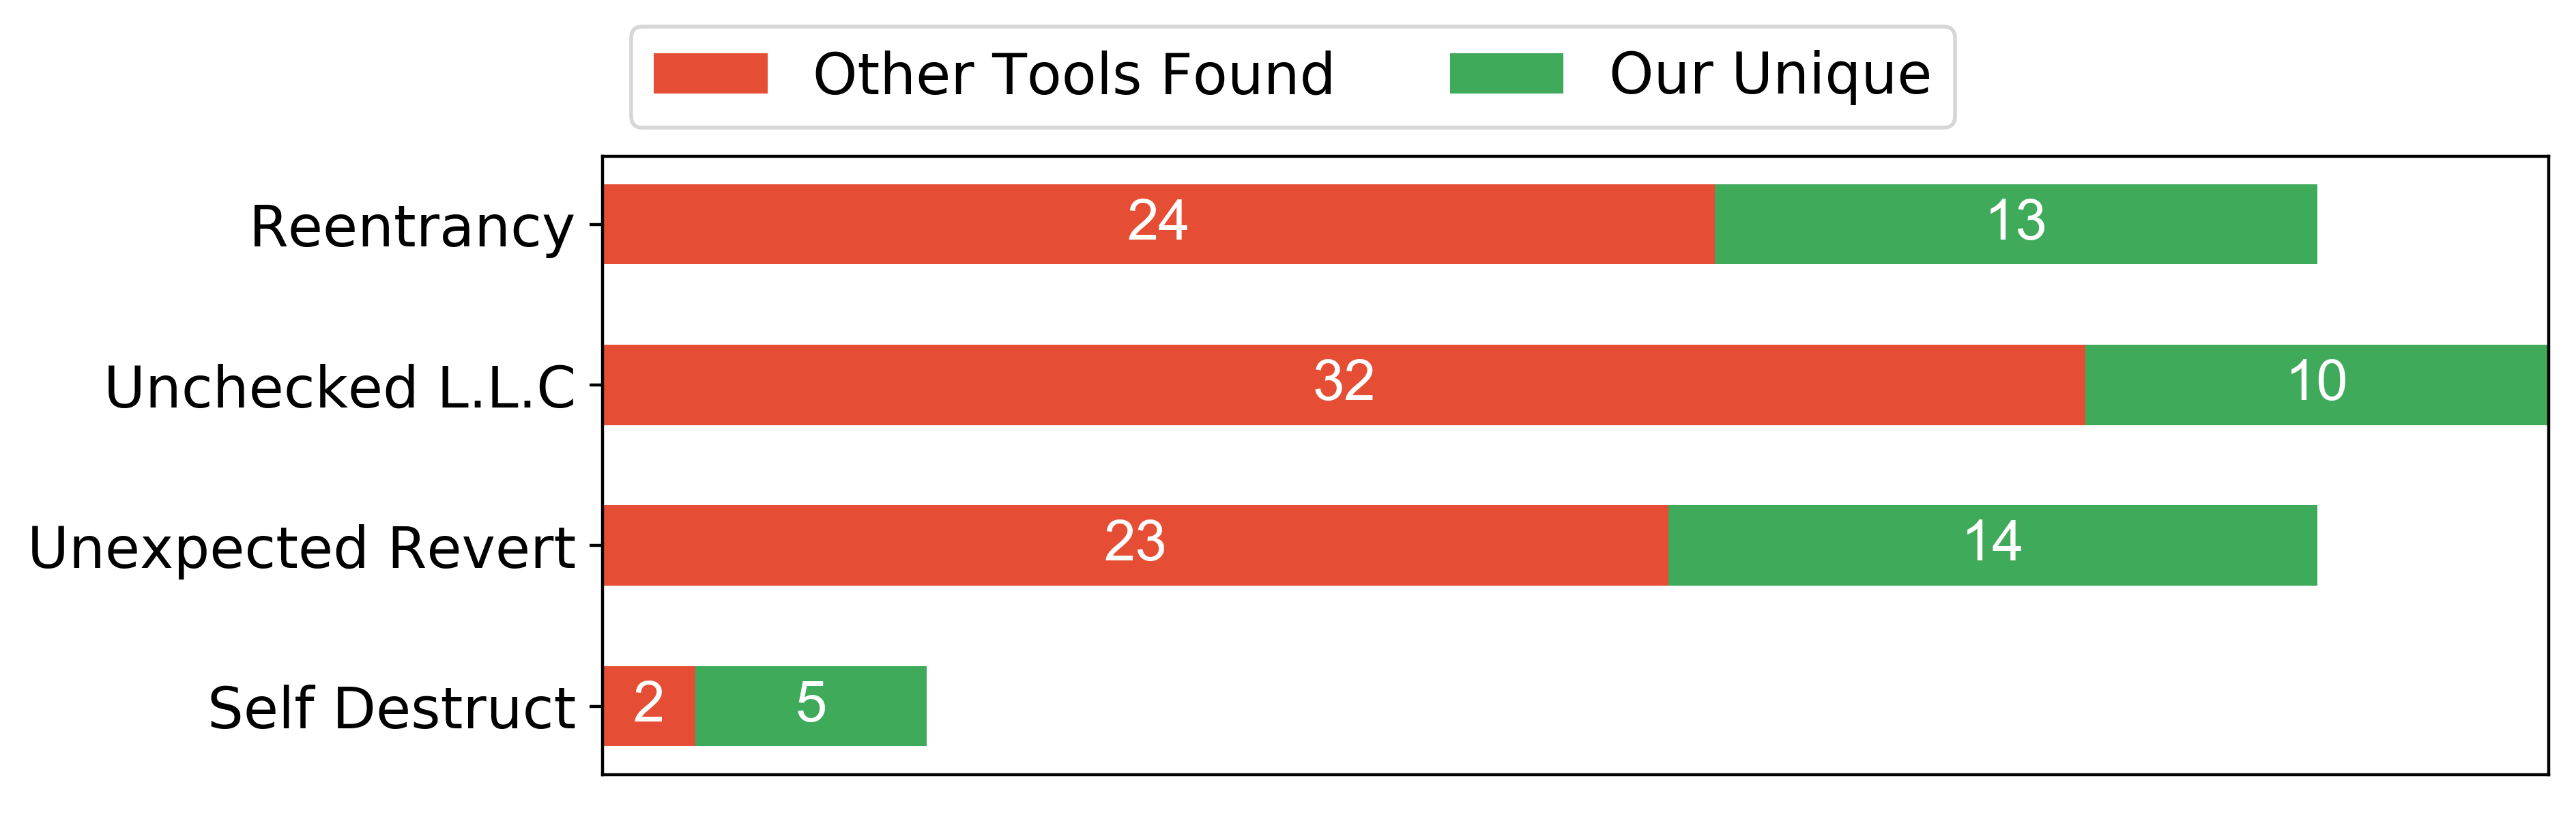
\includegraphics[width=\linewidth]{figures/unique_tp.png}
  \caption{发现的真实漏洞数量统计,“Our Unique”表示只被我们发现的漏洞}\label{fig:unique_tp}
\end{figure}
如图所示,这个标准漏洞库包含了\textcolor{red}{612}个漏洞实例。在这之中,可重入漏洞和低级调用漏洞占了所有漏洞数量可观的比重,其他两个漏洞则较少。在实验完成之后并联系上漏洞关联软件的开发者后,我们会将部分漏洞在网站上进行公开。

\subsubsection{动态验证漏洞的真实性}

为了验证我们在实验中检测到的漏洞的真实性,我们对漏洞实例进行了简单的随机采样,并试图在我们的本地环境进行漏洞的触发。特别地,我们针对每个漏洞签名采样2个漏洞进行测试,只选用两个漏洞是因为使用漏洞签名匹配的可疑代码大多相似,如果测试代码被成功出发,则这些相似的代码也能用类似的测试方式进行触发;还有个原因是每次测试所需要的测试用例都需要我们的领域专家进行独立设计,如果需要进行测试的实例太多,会有大量的时间消耗。测试的环境采用了\textsc{Remix}本地环境进行测试。至于如何使用自动化流程进行软件代码测试,或者如何保证测试的高效性和有效性,这些问题超出了本课题研究的范围,不作讨论。

\subsection{RQ2:分析各检测系统的检测结果}

在上一章第\ref{sec:detection_rules}节和第\ref{sec:ss}节中,我们讨论了漏洞签名的归纳总结过程和9中安全盾技术的特点。为了分析这些漏洞签名和安全盾的有效性,我们将17770个未使用的智能合约软件用作测试集,在测试集上使用各种前沿工具以及我们的检测系统进行实验,最后比对检测结果。在统计时,我们将每个工具报告的漏洞都经过了人工专家的审计,这使得我们认为的漏洞代码数据是具备一定可信度的。各个工具在各个漏洞上的检测准确率如表\ref{tab:eval_reentrancy}、\ref{tab:eval_revert}、\ref{tab:eval_llc}、\ref{tab:eval_selfdestruct}所示。

\begin{table}[htbp]
  \centering
  \begin{minipage}[t]{0.48\textwidth}
  \caption{可重入漏洞检测结果}
    \begin{tabular}{cccc}
    \toprule
    Tools & \#N & P\% & R\% \\
    \midrule
    Slither v0.6.4 & 79    & 18.98\%     & 3 \\
    Oyente v0.2.0 & 19  & 10.53\%     & 3 \\
    Smartcheck v0.2.0 & $\times$     & $\times$  & $\times$  \\
    Securify v0.1.0 &  261    & 4.59\%  & 3 \\
    Athena & 58   & 27.59\%     & 3 \\
    \bottomrule
    \end{tabular}%
  \label{tab:eval_reentrancy}%
  \end{minipage}
  \begin{minipage}[t]{0.48\textwidth}
    \caption{意外异常漏洞检测结果}
    \begin{tabular}{cccc}
    \toprule
    Tools & \#N & P\% & R\% \\
    \midrule
    Slither v0.6.4 & 137  & 10.95\%   & 3 \\
    Oyente v0.2.0 & $\times$ & $\times$  & $\times$ \\
    Smartcheck v0.2.0 & 29  & 65.52\%   & 3 \\
    Securify v0.1.0 & $\times$  & $\times$  & $\times$ \\
    Athena & 43   & 79.07\%     & 3 \\
    \bottomrule
    \end{tabular}%
  \label{tab:eval_revert}%
  \end{minipage}
  \begin{minipage}[t]{0.48\textwidth}
    \caption{低级调用漏洞检测结果}
    \begin{tabular}{cccc}
    \toprule
    Tools & \#N & P\% & R\% \\
    \midrule
    Slither v0.6.4 & 18   & 100.00\%     & 3 \\
    Oyente v0.2.0 & $\times$ & $\times$ & $\times$ \\
    Smartcheck v0.2.0 & 91     & 45.05\%     & 3 \\
    Securify v0.1.0 & $\times$ & $\times$ & $\times$ \\
    Athena &  38  & 89.47\%    & 3 \\
    \bottomrule
    \end{tabular}%
  \label{tab:eval_llc}%
  \end{minipage}
  \begin{minipage}[t]{0.48\textwidth}
    \caption{自毁漏洞检测结果}
    \begin{tabular}{cccc}
    \toprule
    Tools & \#N & P\% & R\% \\
    \midrule
    Slither v0.6.4 & 10    & 20.00\%    & 3 \\
    Oyente v0.2.0 & $\times$ & $\times$ & $\times$ \\
    Smartcheck v0.2.0 & $\times$ & $\times$ & $\times$ \\
    Securify v0.1.0 & $\times$  & $\times$ & $\times$ \\
    Athena & 30    & 20.00\%     & 3 \\
    \bottomrule
    \end{tabular}%
  \label{tab:eval_selfdestruct}%
  \end{minipage}
\end{table}%


